% !TEX program = pdflatex
% !TEX encoding = UTF-8
% !BIB program = bibtex
% !TEX spellcheck = en_US
\documentclass[13pt,aspectratio=169]{beamer}

\usetheme{Berkeley}
\usecolortheme{seagull}
\makeatletter
\beamer@headheight=1.5\baselineskip
\makeatother
\addtobeamertemplate{navigation symbols}{}{%
	\usebeamerfont{footline}%
	\usebeamercolor[fg]{footline}%
	\hspace{1em}%
	\insertframenumber/\inserttotalframenumber
}
\setbeamertemplate{caption}[numbered]

\usepackage{amsmath}
\usepackage{amsfonts}
\usepackage{amssymb}
\usepackage{graphicx}
\usepackage[version=4]{mhchem}
\usepackage{siunitx}
\usepackage[superscript,biblabel]{cite}
\usepackage{caption}

\newcommand*{\rmn}[1]{\romannumeral#1}
\newcommand*{\RMN}[1]{\uppercase\expandafter{\romannumeral#1}}

\author[Qi Zhang et. al.]{\underline{Qi Zhang} \inst{1} \and Tian Qin \inst{2} \and Renata Wentzcovitch\inst{1,3} \and Koichiro Umemoto\inst{4}}
\institute{\inst{1} Applied Physics and Applied Mathematics Department, Columbia University, New York, NY \and%
	\inst{2} Department of Earth Sciences, University of Minnesota, Minneapolis, MN \and%
\inst{3} Lamont-Doherty Earth Observatory, Columbia University, Palisades, NY \and%
\inst{4} Earth-Life Science Institute, Tokyo Institute of Technology}
\title[\texttt{qha}]{\texttt{qha}: A Python package for quasi-harmonic free energy calculation for multi-configuration systems\cite{qin2018qha}}
\date{}

\begin{document}

\begin{frame}
	\titlepage
\end{frame}

\section{Introduction}

\subsection{Quasi-harmonic approximation (QHA)}
\begin{frame}{\subsecname}
	\begin{itemize}
		\item QHA is a useful tool to compute materials thermodynamic properties at high temperature and pressure
		\item QHA remains a good approximation up to about $\frac{ 2 }{ 3 }$ of the melting temperature
		\item The combination of ab initio calculation (DFT, DFPT) with QHA can capture both static and vibrational contribution to free energy and other thermodynamic properties
		\item Can deal with systems with multiple structural configurations
	\end{itemize}
\end{frame}

\subsection{Multi-configuration system that \texttt{qha} may apply}
\begin{frame}{\subsecname}
	\begin{itemize}
		\item the order-disorder phase boundary between ice-\RMN{8} and ice-\RMN{7} \cite{umemoto2010order},
		\item the relative stability of hydrous defects in \ce{Mg2SiO4}-forsterite at high $P$ and $T$ \cite{qin2018ab},
		\item the effect of disorder and iron concentration on the spin crossover diagram of \ce{Fe^3+}-bearing \ce{MgSiO3}-bridgmanite \cite{shukla2016spin}.
	\end{itemize}
\end{frame}

\subsection{Methods}
\begin{frame}[allowframebreaks]{\subsecname}
	\begin{itemize}
		\item single configuration system: \begin{equation}\footnotesize
			      Z(T, V) = \sum_{n=1}^{N_c} g_n \exp\big( -{E_n(V)}/{k_B T} \big) \prod_{q, m} \frac{\exp(-\hbar \omega/2k_B T)}{1 - \exp(-\hbar \omega/k_B T)}, F(T, V) = -k_B T \ln Z(T, V),
		      \end{equation}
		\item multi-configuration systems: \begin{align}\footnotesize
			      Z_n (T, V_i) & = \exp \big( -{ F_n (T, V_i) }/{ k_B T } \big), \\
			      Z(T, V_i)    & = \sum_{n=1}^{N_c} g_n Z_n (T, V_i),            \\
			      F(T, V_i)    & = -k_B T \ln Z(T, V_i).
		      \end{align}
		\item finite strain equation of state fitting to string $\{F(T, V_i)\}$’s to a continuous function $F(T, V)$
	\end{itemize}

	\begin{figure}
		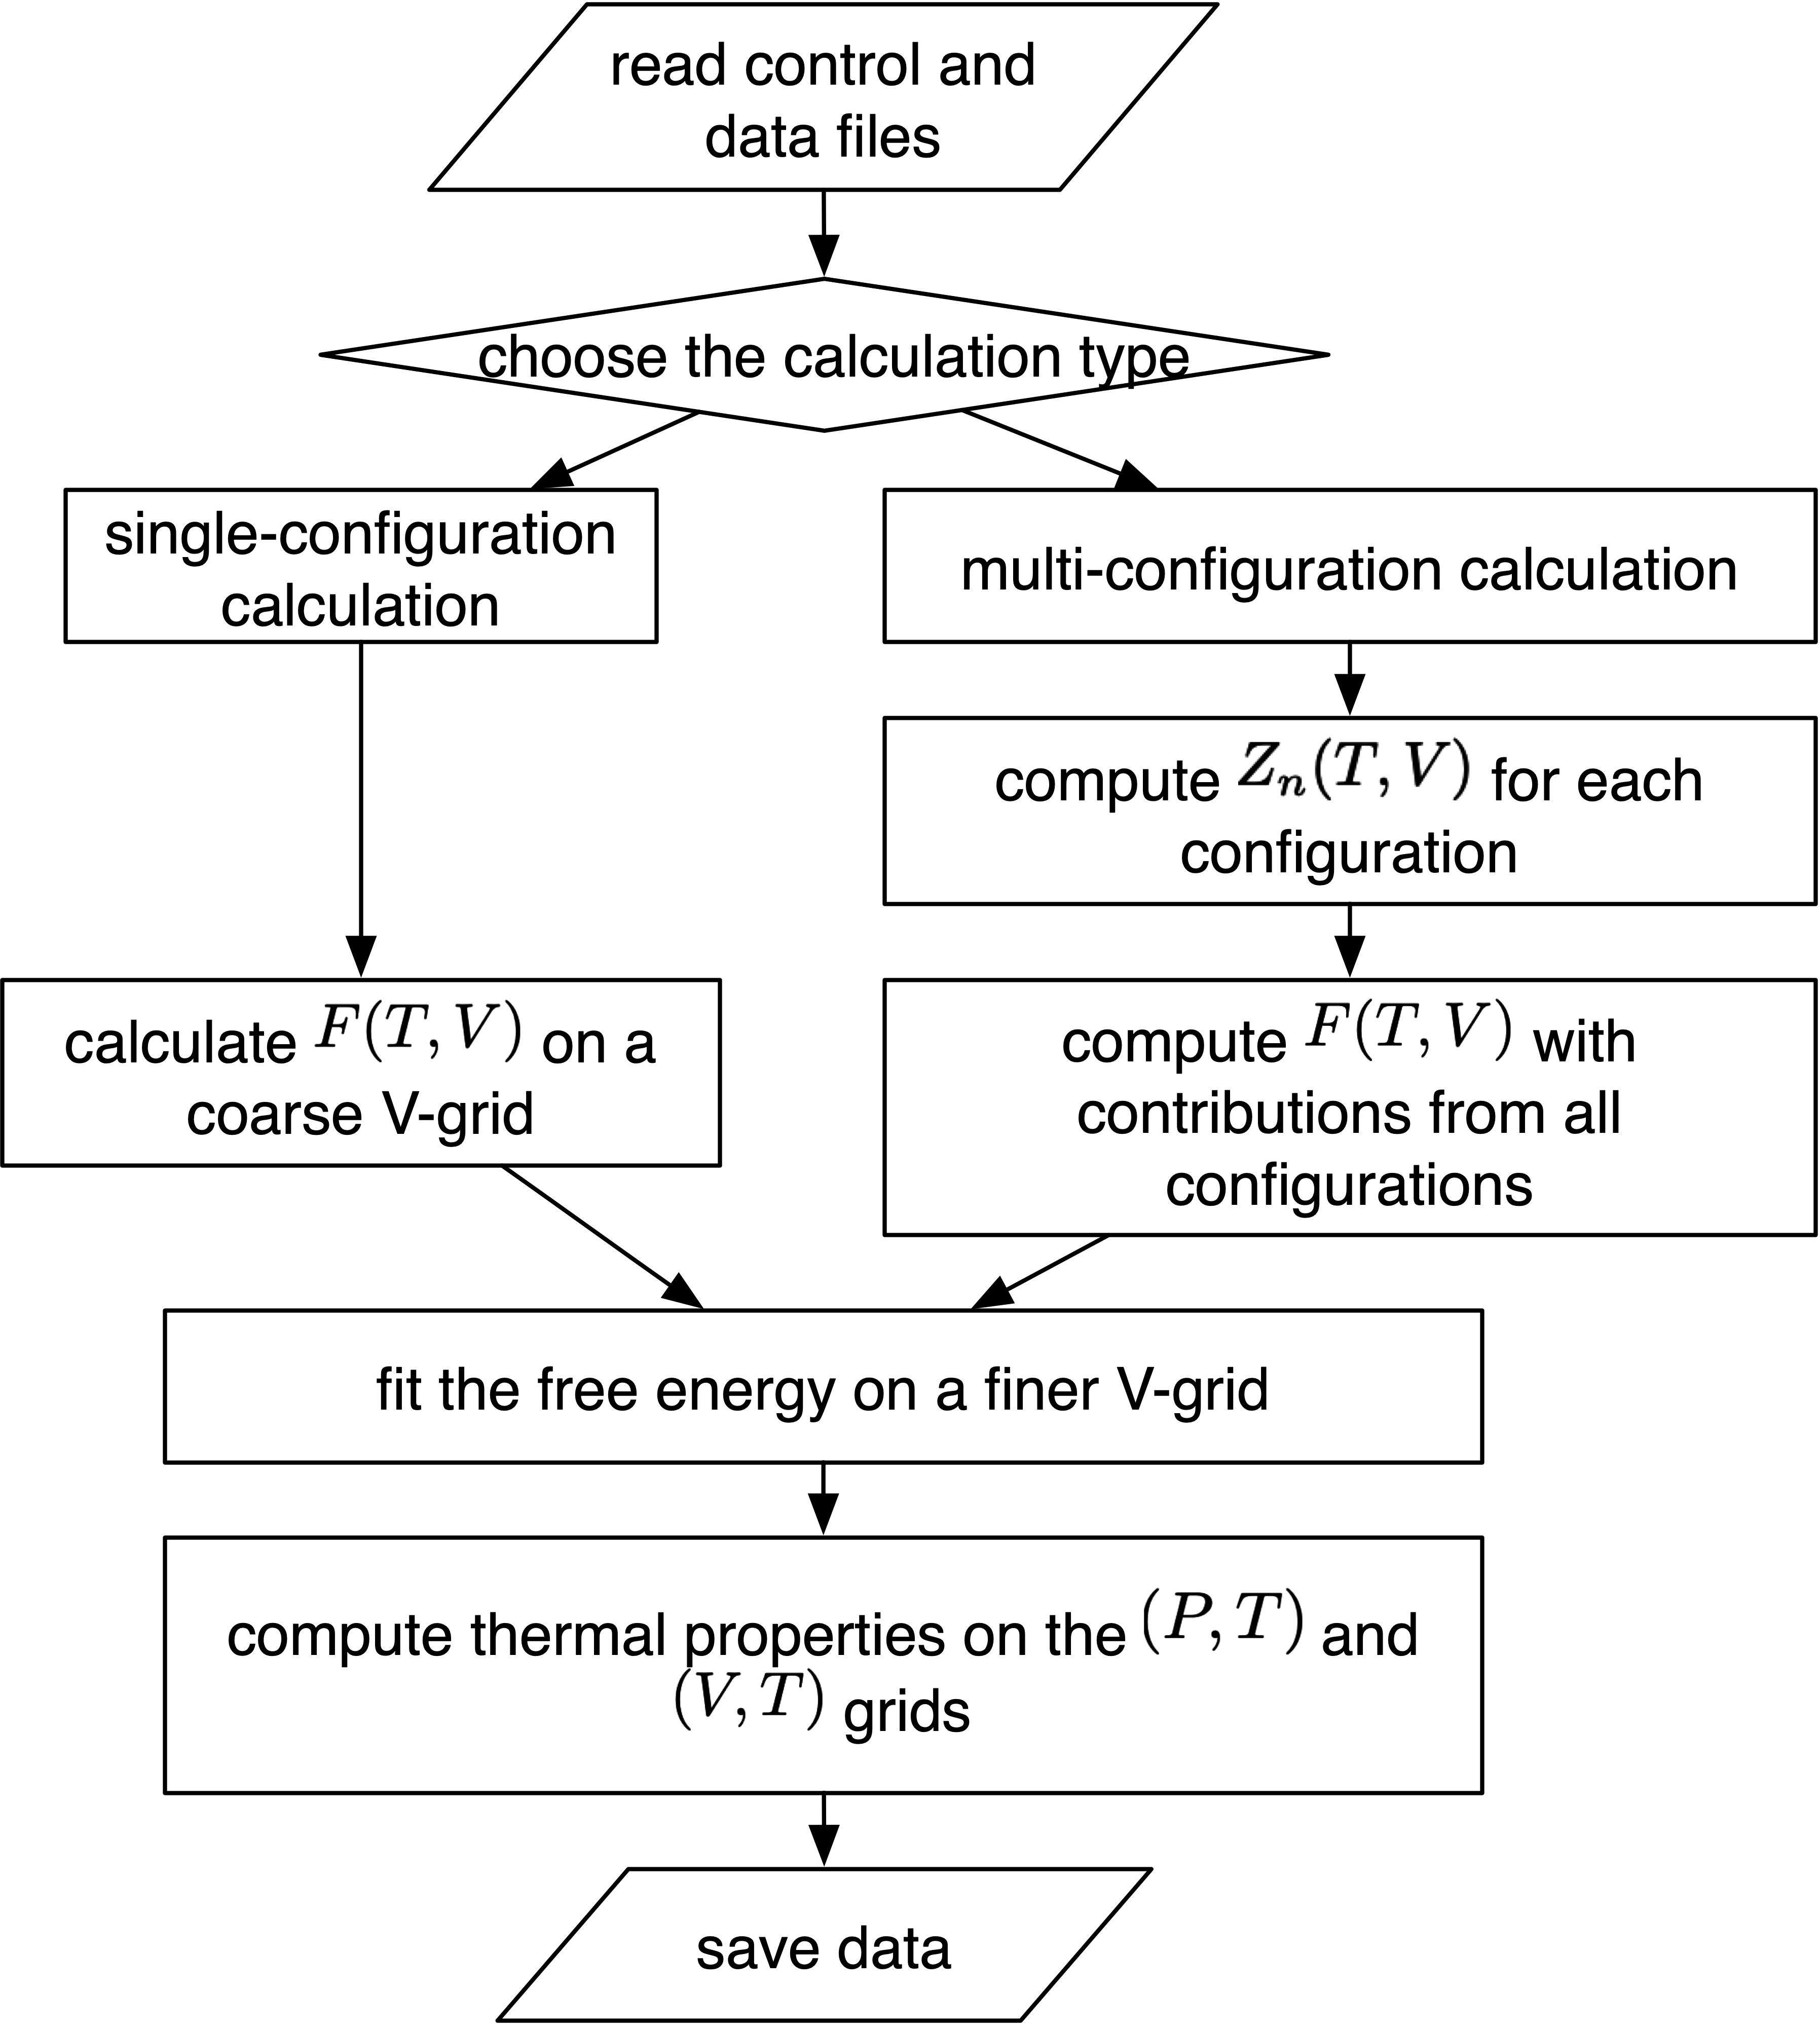
\includegraphics[height=0.8\textheight]{images/flow}%
		\caption{Flowchart of the program}
	\end{figure}
\end{frame}

\section{Examples}

\subsection{ice VII-VIII phase transition}
\begin{frame}[allowframebreaks]{\subsecname}
	\begin{columns}
		\begin{column}{0.5\textwidth}
			\begin{itemize}
				\item The ice Ic has $90$ possible hydrogen configuration, with $4$ symmetrically distinct ones.
				\item The ice \RMN{7} supercell has $8100$ configurations in total, with $52$ symmetrically distinct ones.
				\item Ice \RMN{8} is denoted as the first configuration of ice \RMN{7}.
			\end{itemize}
		\end{column}

		\begin{column}{0.45\textwidth}
			\vspace{\topsep}
			\begin{figure}
				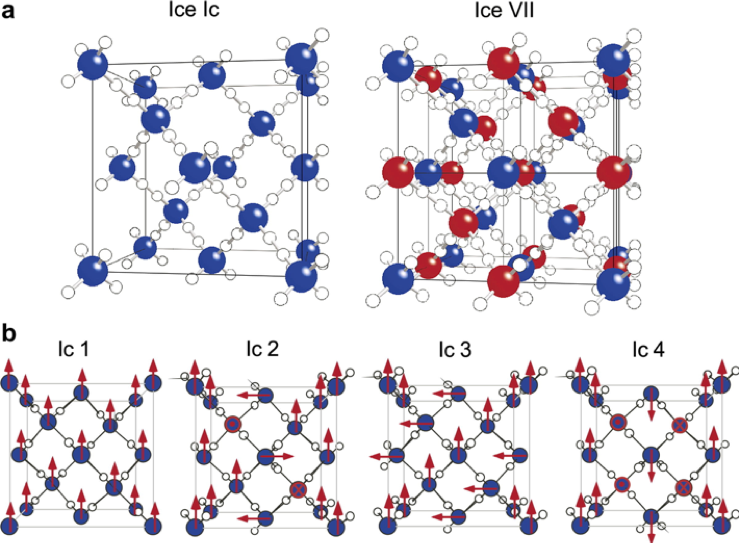
\includegraphics[width=\columnwidth]{images/ice7}%
				\caption{(a) The unit cell of ice Ic and the $2\times 2\times 2$ supercell of ice VII.
					(b) $4$ distinct hydrogen configurations of ice Ic supercells containing $8$ molecules.}
			\end{figure}
		\end{column}
	\end{columns}

	\begin{columns}
		\begin{column}{0.4\textwidth}
			Probabilities of the $52$ symmetrically inequivalent configurations
			generated by the $16$-molecule supercell.
			The contributions from the 2nd to the last configurations
			are not negligible and must be all taken into account.

			\begin{equation*}
				P_i(V, T) = \frac{g_i \exp\Big(\frac{-E_i(V)}{k_B T}\Big)}{Z(V, T)}
			\end{equation*}
		\end{column}

		\begin{column}{0.5\textwidth}
			\vspace{\topsep}
			\begin{figure}
				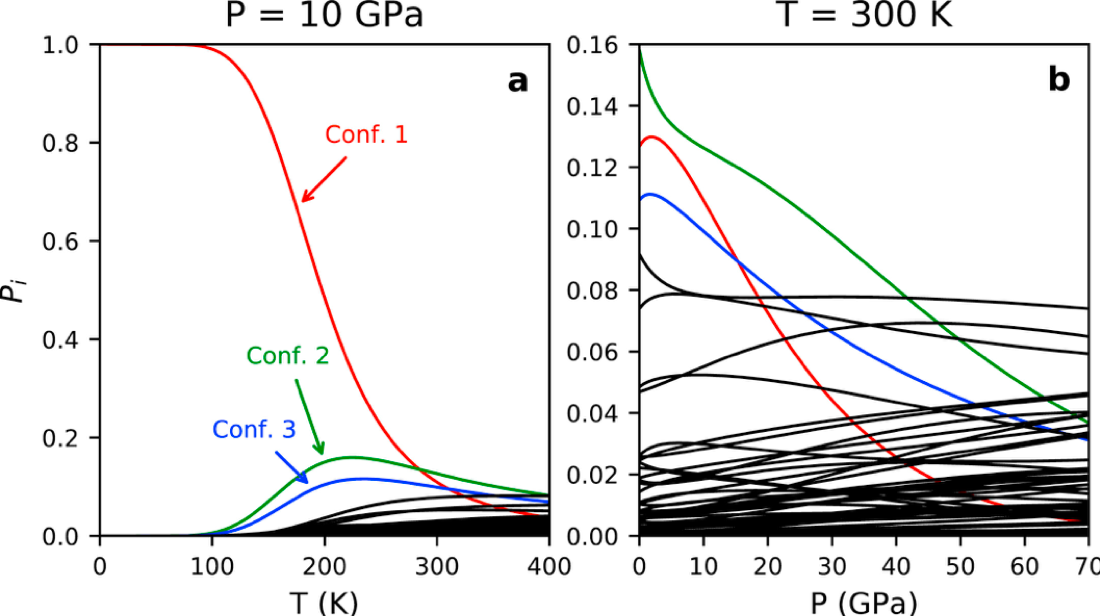
\includegraphics[width=\columnwidth]{images/ice_prob}%
				\caption{Possibilities of each configuration at (a): \SI{10}{\giga\pascal}, (b): \SI{300}{\kelvin}}
			\end{figure}
		\end{column}
	\end{columns}

	\begin{columns}
		\begin{column}{0.45\textwidth}
			\begin{figure}
				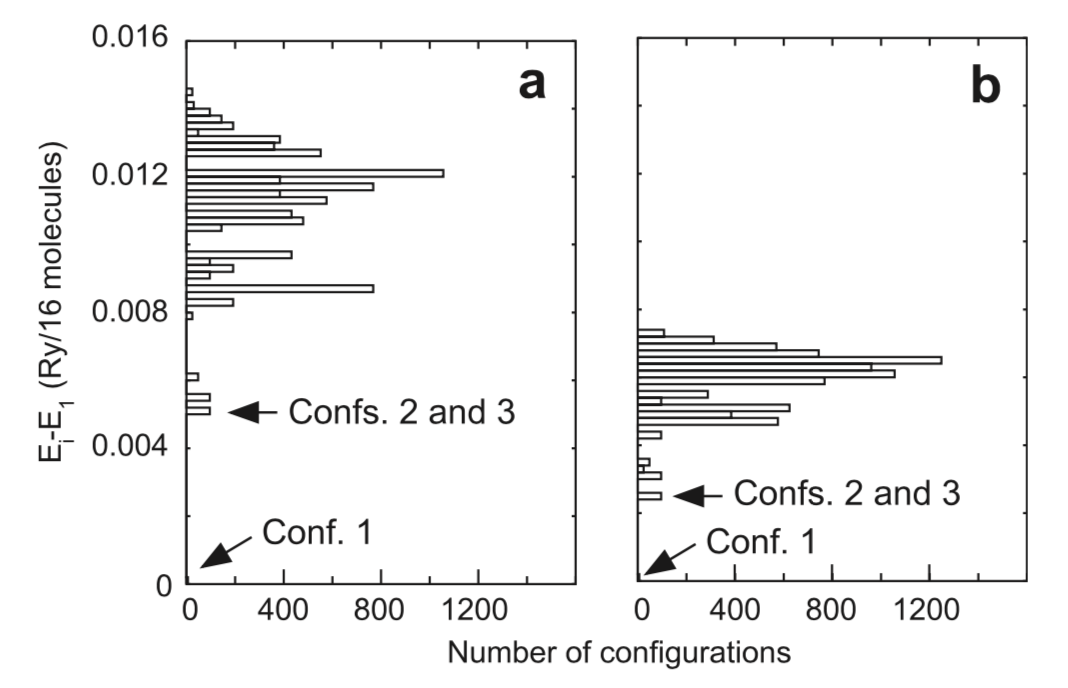
\includegraphics[width=\columnwidth]{images/deltae}%
				\caption{Histograms of the total energy $E_i(V)$ at several volumes at
					(a) \SI{10.32}{\cubic\centi\meter\per\mol} ($\sim$\SI{5}{\giga\pascal}),
					(b) \SI{6.79}{\cubic\centi\meter\per\mol} (\SI{50}{\giga\pascal}).}
			\end{figure}
		\end{column}

		\begin{column}{0.45\textwidth}
			\begin{figure}
				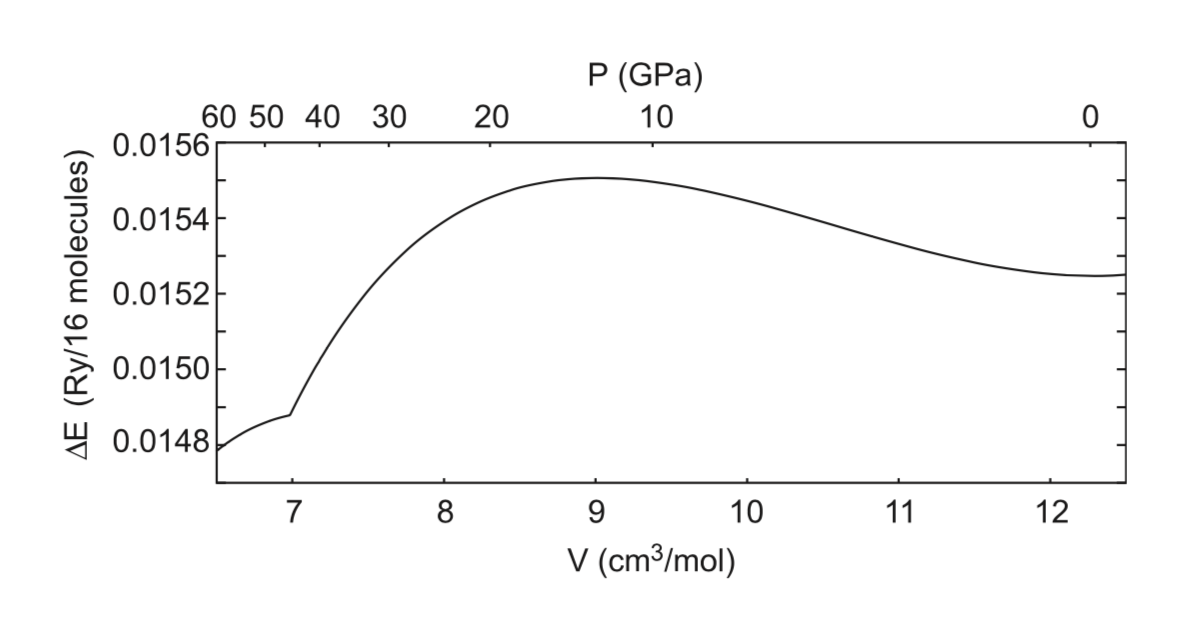
\includegraphics[width=\columnwidth]{images/dltevsp}%
				\caption{Energy distribution: $\Delta E(V) = \max_{1 \leq i \leq 52}[E_i] - \min_{1 \leq i \leq 52}[E_i]$\\
					Clapeyron slope: $\Big( \frac{ \partial T }{ \partial P } \Big)_{ S } = \Big( \frac{ \partial V }{ \partial S } \Big)_{ P } < 0$}
			\end{figure}
		\end{column}
	\end{columns}
\end{frame}

\subsection{stability of hydrous defects in \ce{Mg2SiO4}-forsterite}
\begin{frame}[allowframebreaks]{\subsecname}
	\begin{columns}
		\begin{column}{0.4\textwidth}
			\begin{figure}
				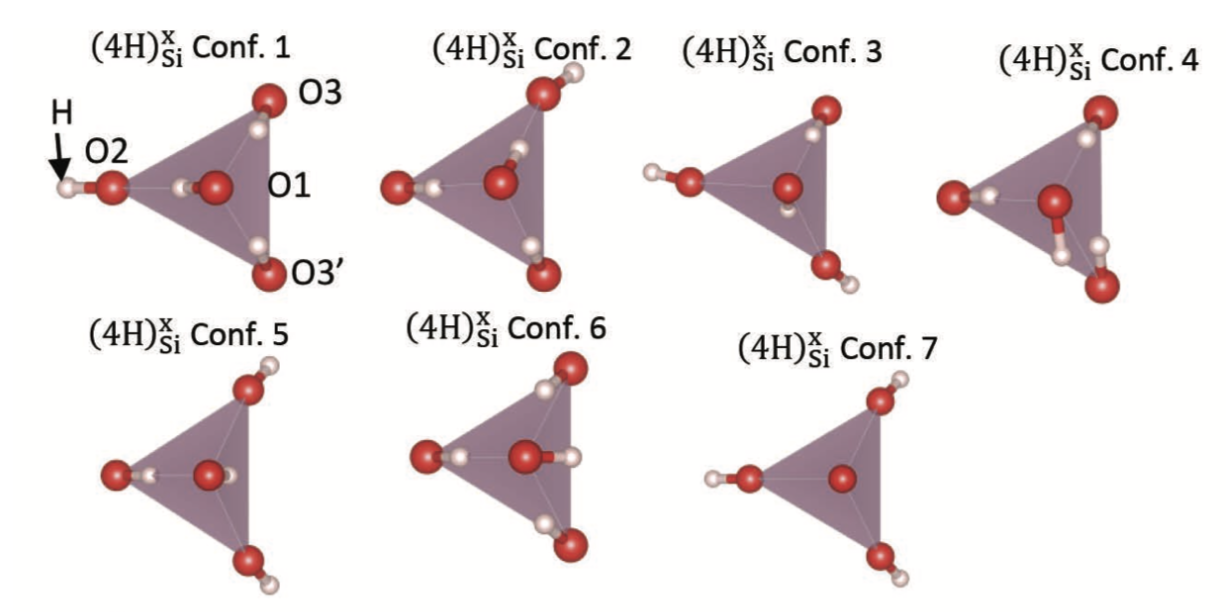
\includegraphics[width=\columnwidth]{images/si}%
				\caption{Configurations of \ce{(4H)^X_{Si}}
				defects. Pink polyhedra represent vacant \ce{Si} sites.}
			\end{figure}
		\end{column}

		\begin{column}{0.4\textwidth}
			\begin{figure}
				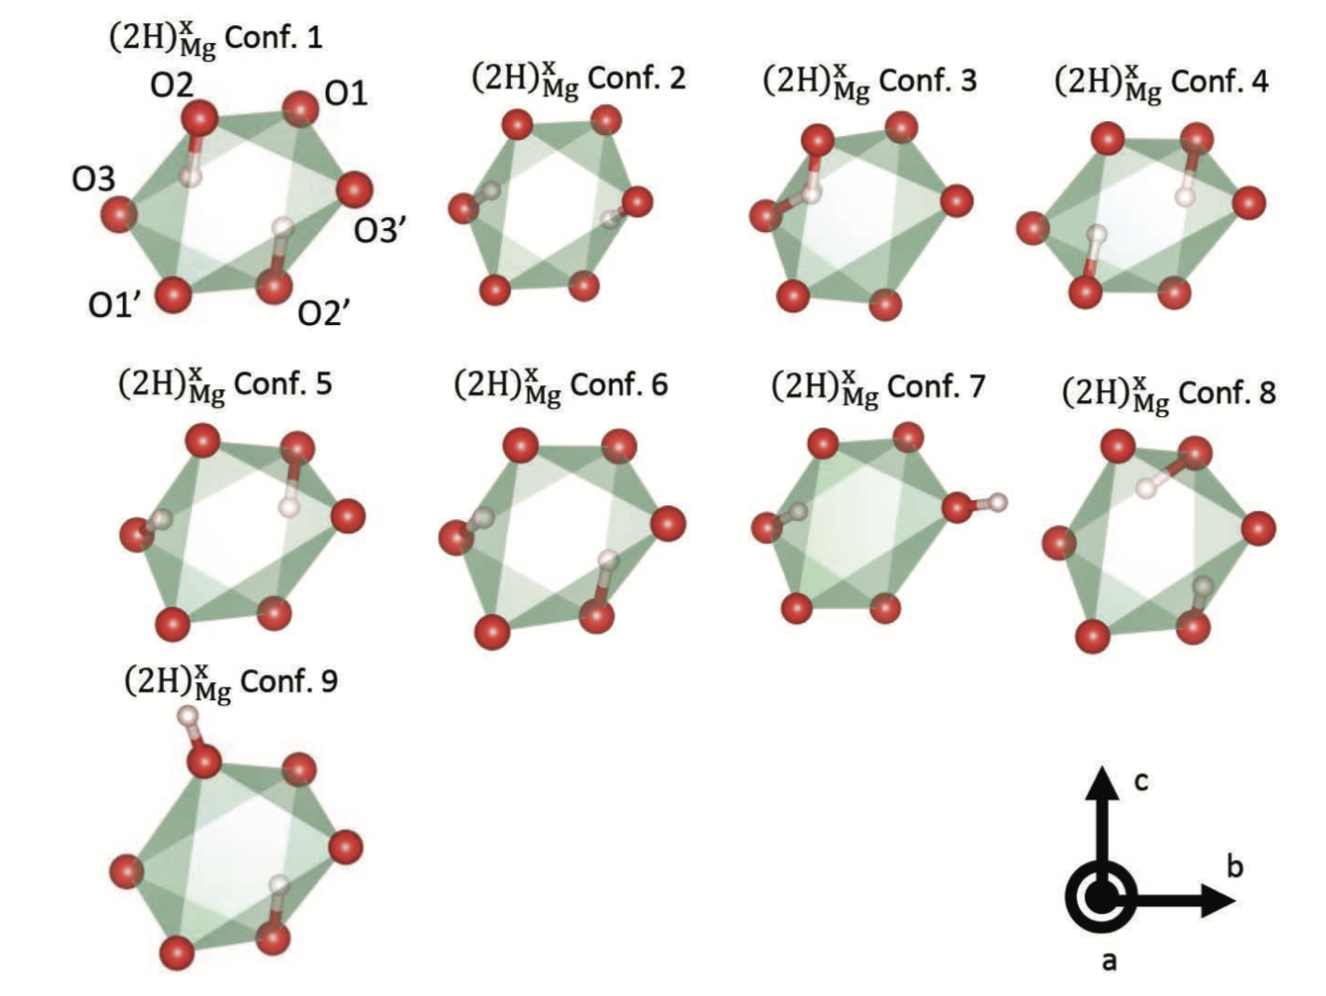
\includegraphics[width=\columnwidth]{images/mg}%
				\caption{Configurations of \ce{(2H)^X_{Mg}}
				defects. Green polyhedra represent vacant \ce{Mg} sites.}
			\end{figure}
		\end{column}
	\end{columns}

	\begin{figure}
		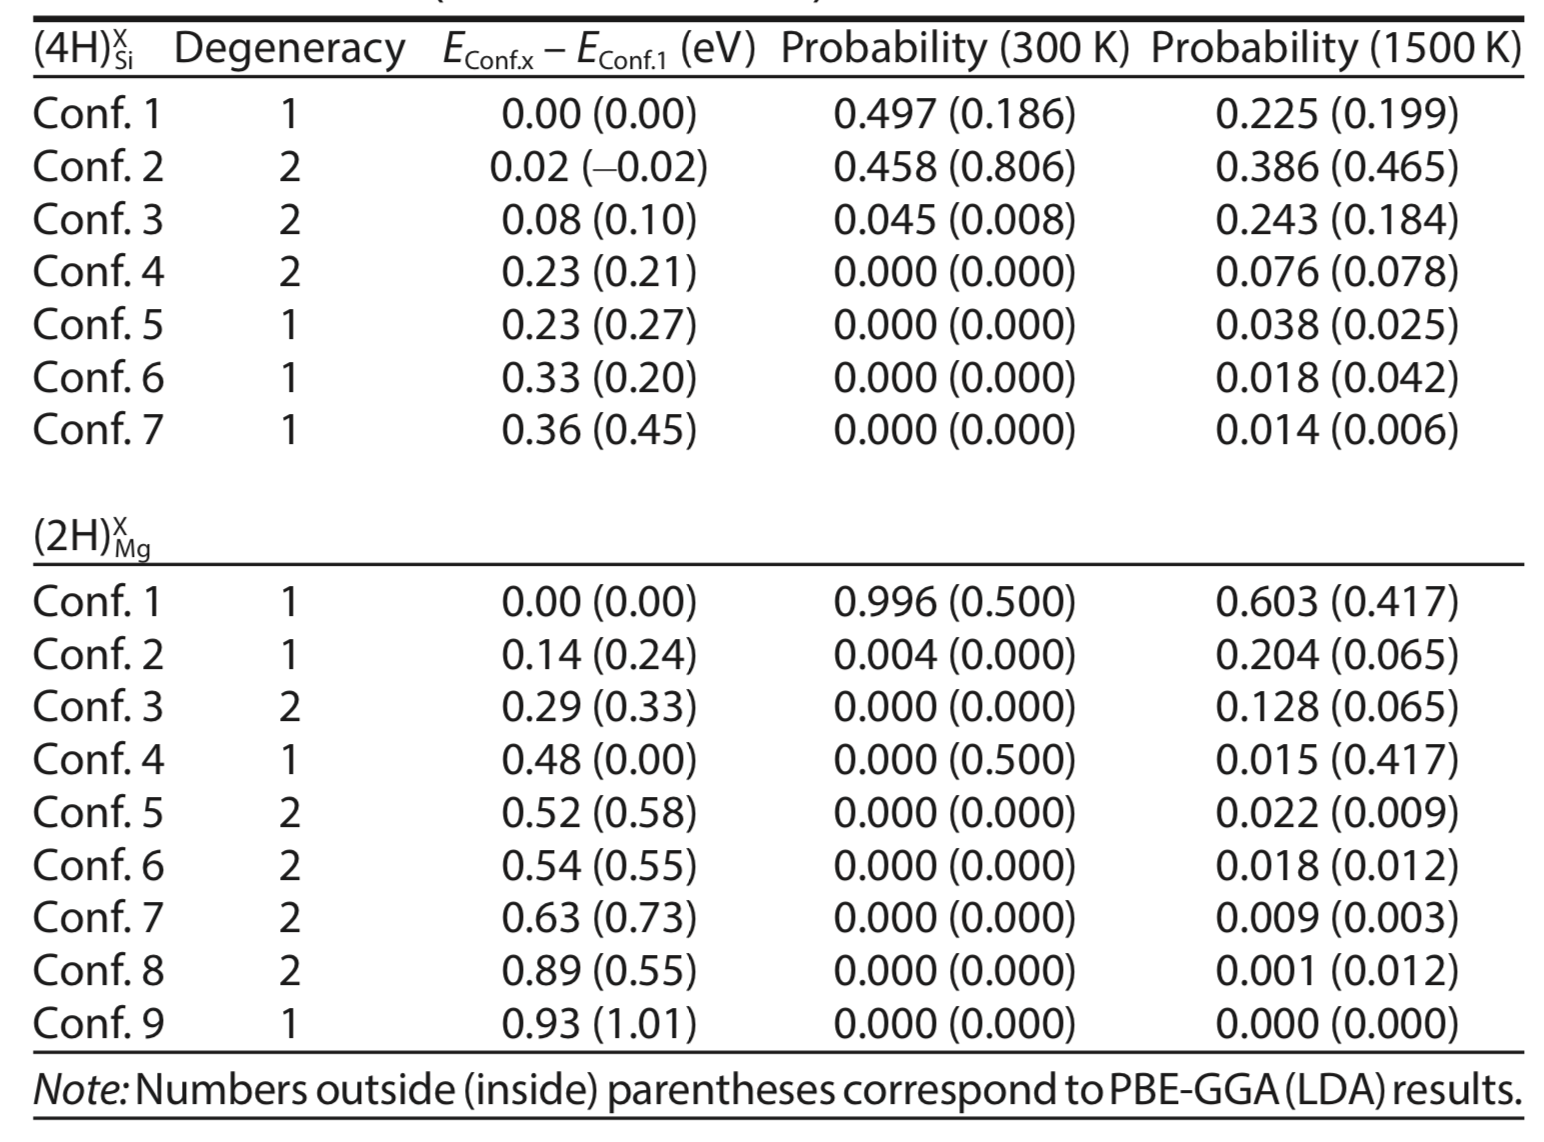
\includegraphics[height=0.6\textheight]{images/simg}%
		\caption{Degeneracies, relative energies, and probabilities of various defects (static calculation)}
	\end{figure}
\end{frame}

\section{Conclusion}

\subsection{Comparisons with other codes}
\begin{frame}{\subsecname}
	\begin{columns}
		\begin{column}{0.45\textwidth}
			\texttt{qha}\\
			\begin{itemize}
				\item $G(T,p) = F(T, V) - \Big( \frac{ \partial F }{ \partial V } \Big)_T V$
				\item directly sample the free energy in Brillouin zone
				\item addresses multi-configuration systems
				\item has command line interface for running and drawing
				\item uses JIT techniques to speedup computation
			\end{itemize}
		\end{column}

		\begin{column}{0.45\textwidth}
			other codes\\
			\begin{itemize}
				\item $G(T,p)= \min_{V}[F(T,V)+pV]$ \cite{phonopy}
				\item integrate the vibrational density of states $g(\omega)$ to get $F$ \cite{Petretto:2018gg}
				\item address the thermodynamic properties of single configuration systems
				\item command line interfaces are not very convenient
				\item Some also are Python, but are slow
			\end{itemize}
		\end{column}
	\end{columns}
\end{frame}

\subsection{Applications to geophysical and mineralogy research}
\begin{frame}{\subsecname}
	\begin{columns}
		\begin{column}{0.45\textwidth}
			\begin{figure}
				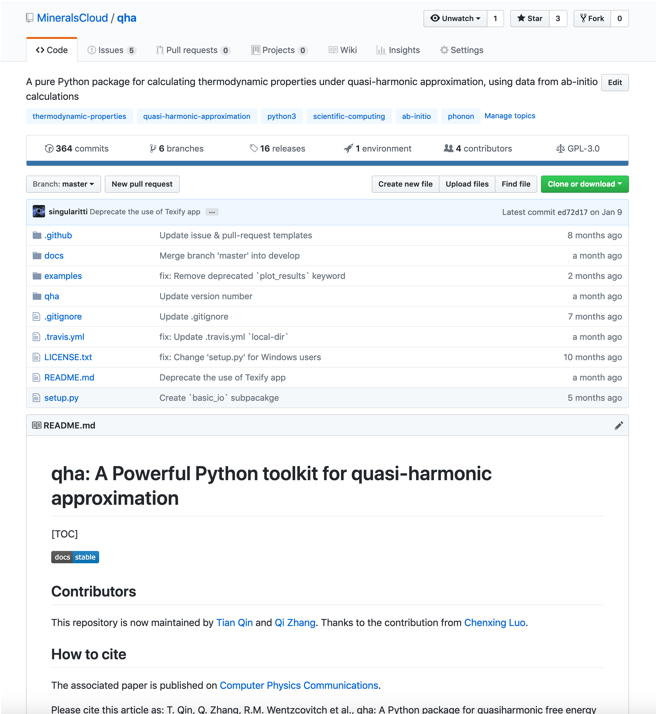
\includegraphics[height=0.8\textheight]{images/website}%
				\captionsetup{labelformat=empty}
				\caption{\scriptsize\url{https://github.com/MineralsCloud/qha}}
			\end{figure}
		\end{column}

		\begin{column}{0.45\textwidth}
			\begin{itemize}
				\item can be extended to investigate thermoelastic properties of materials \cite{Wu:2011ea}
				\item can be extended to investigate metals with its phonon frequencies varying at different temperature
				\item combine with geothermpy code to calculate the geotherm and isentrope \cite{Cardona:2017dd}
				\item can combine with \texttt{rfpr} code to calculate the isotope fractionation factor
			\end{itemize}
		\end{column}
	\end{columns}
\end{frame}

\section{References}
\begin{frame}[allowframebreaks]{\secname}
	\bibliographystyle{unsrt}
	\bibliography{ref}
\end{frame}

\begin{frame}{Acknowledgement}
	\begin{itemize}
		\item NSF EAR-1503084, NSF EAR-1341862, NSF EAR-1348066
		\item Stampede2 at the Texas Advanced Computing Center (TACC), University of Texas at Austin
	\end{itemize}
\end{frame}

\end{document}